\section{Progettazione del database}
\subsection{Schema ER}

\begin{adjustwidth}{-5cm}{-5cm}
    \vspace{\fill}
    \begin{center}
        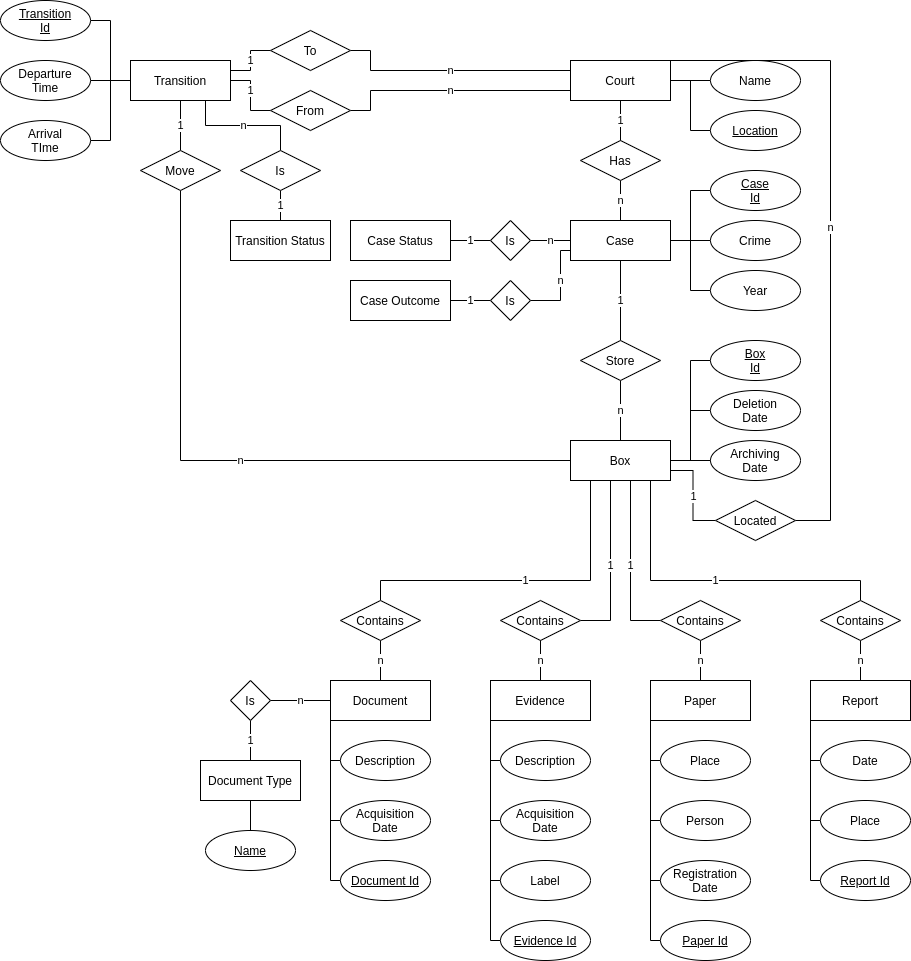
\includegraphics[scale=0.50]{./images/er.png}
    \end{center}
    \vspace{\fill}
\end{adjustwidth}

\subsection{Ipotesi}

\begin{itemize}
    \item Non possono essere eliminati elementi singoli all'interno di una scatola, ma è necessario eliminare la scatola intera.
\end{itemize}

\subsection{Mapping}

Court(\underline{Location}, name, password) \\
Case(\underline{CaseId}, \textit{Court}, \textit{Status}, \textit{Outcome}, Crime, Year) \\
CaseStatus(\underline{Name}, Description) \\
CaseOutcome(\underline{Name}, Description) \\
Box(\underline{BoxId}, \textit{Case}, \textit{Location}, ArchivingDate, DeletionDate)

\noindent \\
Evidence(\underline{EvidenceId}, \textit{Box}, Description, AcquisitionDate, Label) \\
Paper(\underline{PaperId}, \textit{Box}, Place, PersonCF, RegistrationDate) \\
Report(\underline{ReportId}, \textit{Box}, Place, Date) \\
Document(\underline{DocumentId}, \textit{Box}, \textit{Type}, Description, AcquisitionDate) \\
DocumentType({\underline{Name})

\noindent \\
Transition(\underline{TransitionId}, \textit{Box}, \textit{From}, \textit{To}, \textit{Status}, DepartureTime, ArrivalTime) \\
TransitionStatus(\underline{Name}, Description)

\subsection{Normalizzazione}

\subsubsection{Prima forma normale}

Tutte le tabelle sono in prima forma normale, in quanto tutti i campi sono in forma atomica e ogni tabella ha una chiave primaria definita.

\subsubsection{Seconda forma normale}

Tutte le tabelle sono in seconda forma normale, in quanto non esistono campi non chiave che dipendono da una porzione di una chiave candidata composta.

\subsubsection{Terza forma normale}

Tutte le tabelle sono in terza forma normale, in quanto non esistono campi non chiave che dipendono da campi non chiave

\subsubsection{Forma normale di Boyce-Codd}

Tutte le tabelle sono nella forma normale di Boyce-Codd, in quanto tutti i campi determinanti sono superchiavi.

\subsection{Tabelle enumerabili}

Alcune tabelle hanno dei valori fissi ed enumerabili.

\subsubsection{Transition status}
\begin{center}
    \begin{tabular}{c|l}
        \toprule
        \textbf{Value} &
        \textbf{Description}                                           \\
        \midrule
        Requested      & The destintion court requested the transition \\
        Accepted       & The origin court accepted the transition      \\
        Transiting     & The transition is taking place                \\
        Completed      & The transition is completed                   \\
        \bottomrule
    \end{tabular}
\end{center}

\subsubsection{Case status}
\begin{center}
    \begin{tabular}{c|l}
        \toprule
        \textbf{Value} &
        \textbf{Description}                                    \\
        \midrule
        Preliminary    & Preliminary stage                      \\
        First          & Takes place before the court           \\
        Second         & Takes place before the court of appeal \\
        Third          & Takes place in cassation               \\
        Canceled       & The case is no longer active           \\
        \bottomrule
    \end{tabular}
\end{center}

\subsubsection{Case outcome}
\begin{center}
    \begin{tabular}{c|l}
        \toprule
        \textbf{Value} &
        \textbf{Description}                            \\
        \midrule
        Condemned      & The accused has been condamned \\
        Acquitted      & The accused has been aquitted  \\
        \bottomrule
    \end{tabular}
\end{center}

\section{Creazione del database}

Per la creazione del database è stato riportato il mapping in inguaggio SQL. La mappatura completa può essere consultata nel file ``code/sql/db.sql'', mentre sotto è riportato un esempio.

\subsection{Tabella di esempio}

Segue l'implementazione commentata della creazione della tabella ``Box'' in linguaggio SQL per il server MySQL:
\begin{lstlisting}[language=sql]
    CREATE TABLE 'Box' (
        -- inserimento dei campi
        'BoxId' int(11) NOT NULL AUTO_INCREMENT,
        'CaseT' int(11) NOT NULL,
        'Location' varchar(2) NOT NULL,
        'ArchivingDate' date NOT NULL,
        'DeletionDate' date DEFAULT NULL,
        'DeletionReport' TEXT DEFAULT NULL,

        -- keys
        PRIMARY KEY ('BoxId'),
        FOREIGN KEY ('CaseT') REFERENCES 'CaseT' ('CaseId'),
        FOREIGN KEY ('Location') REFERENCES 'Court' ('Location'),

        -- checks
        CHECK (
            'DeletionDate' IS NULL 
            OR YEAR('DeletionDate') - YEAR('ArchivingDate') >= 50
        ),
        CHECK (
            'DeletionDate' IS NULL 
            OR 'DeletionReport' IS NOT NULL
        )
    );
\end{lstlisting}

\subsubsection{Inserimento di dati}

Durante la creazione delle tabelle enumerabili (vedi sezione 6.5) è stata implementato anche l'inserimento dei valori possibili. Segue l'esempio della tabella ``TransitionStatus'':
\begin{lstlisting}[language=sql]
    INSERT INTO 'TransitionStatus' ('Name', 'Description') VALUES
        ('Accepted', 'The destintion court requested the transition'),
        ('Completed', 'The origin court accepted the transition'),
        ('Requested', 'The transition is taking place'),
        ('Transiting', 'The transition is completed');
\end{lstlisting}

\section{Queries aggiuntive}

Le tre queries aggiuntive sono consultabili nella cartella ``code/sql/queries''. La query 3 non può essere eseguita con un'interrogazione sola, ma è possibile ottentere il risultato desiderato con 4 interrogazioni separate.

\section{Applicazione WEB}

Il codice dell'applicazione WEB è consultabile nella cartella ``code/web''.

\subsection{Login}

Per autenticare il login è necessario inserire una password, della quale solo il digest MD5 è salvato nel database. Le password di default sono uguali alla locazione del tribunale: ad esempio, la password del tribunale di CN (Cuneo) è `CN'.

\subsection{Funzioni mancanti}

I link che richiedono funzioni non implementate redirigono ad una pagina che indica chiaramente lo stato di ``lavori in corso''. Alcune features sono mancanti ma non indicate da nessun link specifico:

\paragraph{Modifica dei casi}
Manca la possibilità di modificare i campi, la quale permetterebbe di fare uso dei campi di ``status'' e ``outcome''.

\paragraph{Informazioni aggiuntive}
Al contrario che per gli items, non è al momento possibile vedere informazioni agginutive sui casi e sulle scatole.

\subsection{Grafica}
L'aspetto grafico è stato curato con HTML e CSS personalizzato, consultabile nella cartella ``code/web/css''.

\subsection{Paginazione}
Per poter implementare un sistema di paginazione che permettesse la non ripetizione del codice è stato necessario dividere il programma monolitico PHP in diverse pagine (nella cartella ``code/web/partials'') che sono renderizzate dallo spezzone di codice:
\begin{lstlisting}[language=php]
    $pages = [ ... ];
    $page = $_GET['page'];
    if ( in_array($page, $pages))
        require('../partials/' . $_GET['page'] . '.php');
\end{lstlisting}
che permette di indicare la pagina desiderata tramite il parametro URI ``page'' (eg. ?page=local) e, se la pagina richiesta è presente nella lista di pagine aturizzate, viene renderizzata. Ciò permette inoltre ai browser moderni applicare solo le nuove modifiche alla pagina HTML, velocizzando il caricamente e rendendo l'esperienza per l'utente più piacevole.
